% resume.tex
% Adithya Balaji

% Start a document with the here given default font size and paper size.
\documentclass[10pt,letterpaper]{article}
% \documentclass[10pt,letterpaper,twocolumn]{article}

% Set the page margins.
\usepackage[letterpaper,left=0.25in,right=0.25in,top=0.25in,bottom=0.25in]{geometry}

% Setup the language.
\usepackage[english]{babel}

% Makes resume-specific commands available.
\usepackage{resume}

% Optinally show/hide the image
% \toggletrue{hideimage}

\begin{document}  % begin the content of the document
\sloppy  % this to relax whitespacing in favour of straight margins

% header.tex

% title on top of the document

\newcommand{\website}[1]{\href{}}{}

% Main content
\newcommand{\headerinfo}{%
	%\vspace{-2cm}
	\maintitle{Adithya Balaji}
	\vspace{0.4em}\\
	\textsmaller{+}1 (919)--656--2815\sbull{}
	\href{mailto:adithyabsk@gmail.com}{adithyabsk\mbox{}@\mbox{}gmail.com}\sbull{}
	\href{https://github.com/adithyabsk}{github://adithyabsk}\sbull{}
	\href{https://linkedin.com/in/adithyabsk}{linkedin://adithyabsk}
	\vspace{0.4em}\\
	Raleigh\sbull{}
	North Carolina
	% \nobreakvspace{0.3em}  % add some page break averse vertical spacing
}

% \null \vfill make sure that the image is centered with the multicols text
% Modify columnsep to accomodate image and set back to default value
\newcommand{\headercontent}[3]{%
	\iftoggle{hideimage}{%
		\headerinfo{}\spacedhrule{0.8em}{0.8em}
	}{%
		\setlength{\columnsep}{-44em}
		\vspace{#1}%
		\begin{multicols}{2}
			\hspace{#2} % remove some variable space if single column
			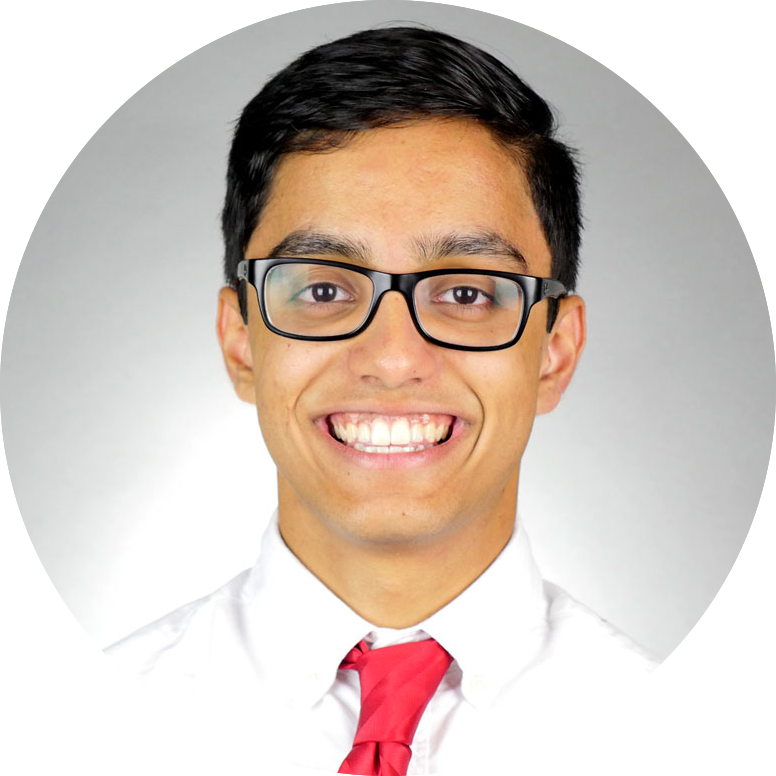
\includegraphics[width=2cm]{headshot}
			\vfill\null\columnbreak{}
			\headerinfo{}
			\headerlinks{}
		\end{multicols}
		\setlength{\columnsep}{10pt}\spacedhrule{-1.6em}{#3}
	}
}

% Some serious space hacking was necessary to make the header remain
% constant between twocols and not twocols
\makeatletter%
\if@twocolumn%
	\twocolumn[
		\headercontent{-0.4cm}{0cm}{0.8em}
	]
\else% \@twocolumnfalse
	\headercontent{0em}{-0.55cm}{-0.6em}
\fi
\makeatother


\roottitle{Work Experience}
% experience.tex

% Links
\newcommand{\foreshadow}[1]{\href{https://github.com/georgianpartners/foreshadow}{#1}}
\newcommand{\gppaperone}[1]{\href{https://github.com/georgianpartners/automl_benchmark}{#1}}
\newcommand{\gppapertwo}[1]{\href{https://arxiv.org/abs/1808.06492}{#1}}
\newcommand{\gppaperthree}[1]{\href{https://assert.pub/papers/1808.06492}{#1}}

\newcommand{\gpblogone}[1]{\href{https://medium.com/georgian-impact-blog/python-tooling-makes-a-project-tick-181d567eea44}{#1}}
\newcommand{\gpblogtwo}[1]{\href{https://medium.com/georgian-impact-blog/choosing-the-best-automl-framework-4f2a90cb1826}{#1}}
\newcommand{\gpblogthree}[1]{\href{https://medium.com/georgian-impact-blog/automatic-machine-learning-aml-landscape-survey-f75c3ae3bbf2}{#1}}

\newcommand{\plone}[1]{\href{https://support.precisionlender.com/hc/en-us/articles/115009642807-Rate-Sheet-Printouts}{#1}}

\newcommand{\bitzer}[1]{\href{https://www.computerhistory.org/events/bio/Donald,Bitzer}{#1}}

\newcommand{\nbahacks}[1]{\href{https://hackathon.nba.com/}{#1}}

\headedsection{\href{https://georgianpartners.com/}{Georgian Partners}}
{\textsc{Toronto, Canada}}
{%
	\headedsubsection{Data Science Intern}
	{May \apo18--Current}
	{%
		\bodytext{%
			Led the development of \foreshadow{Foreshadow}, an open-source Python \mbox{AutoML} package.
			\begin{tightemize}
				\item Architected and developed the tool to automatically build and tune an end-to-end machine learning model that interops \texttt{sklearn} and \texttt{pandas}. (100\% branch test coverage)
				\item Wrote an \gppaperone{extensible AutoML benchmark} package using \texttt{boto3}, \texttt{AWS Batch}, and \texttt{EC2} and an accompanying \gppapertwo{engineering research paper} that gained \gppaperthree{significant Twitter traction}.
				\item \gpblogone{Authored} three \gpblogtwo{Medium blogs} on \gpblogthree{automatic machine learning} and Python tooling that were read 16,000\textsmaller{+} times.
			\end{tightemize}
		}
	}
}

\headedsection{\href{https://www.csc.ncsu.edu/}{Bitzer Lab}}
{\textsc{Raleigh, NC}}
{\headedsubsection{CS Research Assistant}
	{August \apo17--Current}
	{%
		\bodytext{%
			Was advised by \bitzer{Dr.\ Donald Bitzer} \textit{(inventor of plasma screen TV)} in the development of advances in bioinformatics.
			\begin{tightemize}
				\item Upgraded a broken, legacy Python \texttt{django} website.
				\item Implemented an updated version of an mRNA optimization algorithm to increase protein yield.
			\end{tightemize}
		}
	}
}

\headedsection{\href{https://www.nba.com/thunder/}{Oklahoma City Thunder}}
{\textsc{Raleigh, NC}}
{\headedsubsection{Data Science Intern}
	{January \apo19--May \apo19}
	{%
		\bodytext{%
			After a strong performance at the \nbahacks{NBA Hackathon}, I was recruited to develop a basketball shot quality model.
			\begin{tightemize}
				\item Grokked input data using game footage and developed dynamic data visualizations using \texttt{seaborn} and \texttt{bokeh}.
				\item Presented a shot quality model (ROC AUC, 0.92) to team executives that increased downstream accuracy by 1\%.
				\item Delivered a deployable \acr{CLI} to the model that could be rerun yearly to mitigate model drift.
			\end{tightemize}
		}
	}
}

\headedsection{\href{https://precisionlender.com/}{Precision Lender}}
{\textsc{Cary, NC}}
{\headedsubsection{Software Engineering Intern}
	{May \apo17--Aug \apo17}
	{%
		\bodytext{%
			Was invited by the CEO to work on the company's core product: a commercial loan pricing tool.
			\begin{tightemize}
				\item Architected and developed a scalable natural language processing (NLP) system that cached queries using an Azure Service Fabric Stateful microservice. (C\#)
				\item Demoed to the entire company and deployed the solution to production currently used by 100\textsmaller{s} of banks worldwide.
				\item Documented a \plone{major release} and developed a web tooling interface operating on the production database. (Javascript)
			\end{tightemize}
		}
	}
}
%
\spacedhrule{0.5em}{-1.2em}%

\roottitle{Extracurriculars}
% extracurriculars.tex

\headedsection{\href{http://liquidrocketry.com/}{Liquid Rocketry Lab}}
{\textsc{Raleigh, NC}}
{\headedsubsection{Chief Business Officer}
	{Aug \apo18--Current}
	{%
		\bodytext{%
			Founded and developed NC's first liquid propulsion laboratory developing a spacebound rocket (Kármán Line, 100\textsmaller{km})
			\begin{tightemize}
				\item Recruited a talented, diverse core team of 50 students.
				\item Managed a team of 15 students to raise \$250,000. Brokered partnerships with companies such as RedBull and Jacobs.
				\item Managed legal matters including nonprofit registration, tax exempt status and insurance procurement.
			\end{tightemize}
		}
	}
}

\headedsection{\href{http://ewh.ieee.org/sb/nc/ncsu/}{NC State IEEE Chapter}}
{\textsc{Raleigh, NC}}
{\headedsubsection{President, Chair}
	{Aug \apo17--May \apo20}
	{%
		\bodytext{%
			Responsible for the largest professional society at NC State.
			\begin{tightemize}
				\item Established a \$400 scholarship for students in the ECE department
				\item Increased student membership by 20\% (to 400\textsmaller{+} members) by conducting technical talks of interest to members.
				\item Coordinated the yearly student delegation to the South East Regional conference where the team has won 5\textsmaller{+} awards.
				\item Organized the NC State IEEE Extreme Hackathon with significant student participation. (2017, 2018, 2019)
			\end{tightemize}
		}
	}
}

\headedsection{\href{https://ncstatefirstalumni.com/}
	{NC State FIRST Alumni Association}}
{\textsc{Raleigh, NC}}
{\headedsubsection{President}
	{Aug \apo18--May \apo19}
	{%
		\bodytext{%
			Founded and grew North Carolina's first collegiate alumni program for high school robotics participants.
			\begin{tightemize}
				\item Grew the organization to over 70 members in the first year.
				\item Organized a special event with FIRST's founder, Dean Kamen, at NC State.
				\item Empowered students to volunteer for over 1,000 hours across local FIRST robotics events in dire need of help through club funds.
			\end{tightemize}
		}
	}
}

\headedsection{%
	\href{https://www.tbp.org/off/DisplayChapterInfo.cfm?ID=129}{Tau Beta Pi NC Alpha Chapter}
}
{\textsc{Raleigh, NC}}
{%
	\headedsubsection{Vice President}
	{Aug \apo18--May \apo19}
	{%
		\bodytext{%
			Responsible for managing the organization's day-to-day operations of the largest honors society at NC State.
			\begin{tightemize}
				\item Assisted in the organization of professional development and volunteering events for student induction requirements.
				\item Inducted a class of the top 30 students in the engineering department into the prestigious society.
			\end{tightemize}
		}
	}
}

\headedsection{\href{https://team900.org/}{Robotics at NCSSM}}
{\textsc{Durham, NC}}
{%
	\headedsubsection{Team Captain}
	{Aug \apo15--May \apo17}
	{%
		\bodytext{%
			Responsible for delivering strong competition results for one North Carolina's oldest robotics teams.
			\begin{tightemize}
				\item Managed a team of 50 students to fabricate a 120 lb.\ robot in the span of 6 weeks to compete in a yearly challenge.
				\item Successfully spearheaded significant technical advancements in robot perception and control using deep learning and ROS, respectively.
				\item Led the team to a world championship quarterfinal berth and, later, open sourced our winning code.
			\end{tightemize}
		}
	}
}

\headedsection{%
	\href{https://web.archive.org/web/20181221034926/https://www.ncssm.edu/residential-program/academics/sustainability}{Sustainability at NCSSM}
}
{\textsc{Durham, NC}}
{%
	\headedsubsection{Sustainability Project Leader}
	{Aug \apo16--May \apo17}
	{%
		\bodytext{%
			Managed the implementation of the strategic sustainability vision of the school.
			\begin{tightemize}
				\item Created and performed Energy Star portfolio analysis for the school and made recommendations to reduce the carbon footprint.
				\item Converted the cafeteria to a zero waste zone through a partnership with local composting organization, CompostNow.
			\end{tightemize}
		}
	}
}
%
\spacedhrule{0.5em}{-1em}%

\roottitle{Volunteering}
% volunteer.tex

% Hours calculation for FIRST robotics
% 2017 (Steamworks)
%   * THOR - 20 hours
%   * 2017 total hours = 20 hours
% 2018 (Power Up)
%   * Pitt County - 30 hours
%   * Pembroke - 30 hours
%   * Asheville - 30 hours
%   * Forsyth - 30 hours
%   * State Champs - 30 hours
%   * THOR - 20 hours
%   * 2018 total hours = 20+5*30 = 170 hours
% 2019 (Deep Space)
%   * Wake County - 30 hours
%   * Asheville - 30 hours
%   * State Champs - 30 hours
%   * Houston World Champs - 40 hours
%   * 2019 total hours = 3*30+40 = 130 hours
% Total Hours = 20 + 170 + 130 = 320 hours

% Student impact
% 30 students per team, 70 teams ~ NC --> 2100 students
% Turing 66 teams --> ~2000 students

\headedsection{\href{https://www.firstinspires.org/}{FIRST Robotics}}
{\textsc{USA}}
{%
	\headedsubsection{Referee / Field Technical Advisor}
	{Aug \apo17--Current}
	{%
		\bodytext{%
			Responsible for upholding the spirit of gameplay in FIRST robotics events and debugging technical issues on a 52\(\times\)26 ft.\ game-play field.
			\begin{tightemize}
				\item Devoted over 320 hours to serving the high school robotics community spanning the entire State of North Carolina.
				\item Impacted over 4000 students, yearly, across both North Carolina events and the World Championship event where students bring 120 lb.\ robots to compete in the highest level of high school robotics.
			\end{tightemize}
		}
	}
}

\headedsection{\href{http://www.desidancenetwork.org/navarasa}{Navarasa}}
{\textsc{Raleigh, NC}}
{%
	\headedsubsection{Finance Chair}
	{Aug \apo18--Current}
	{%
		\bodytext{%
			Responsible for managing the financial operation and previously technical operations of the North Carolina's largest, Indian classical dance competition.
			\begin{tightemize}
				\item Raised over \$10,000 for CRY, Children's Rights and You, an organization devoted to improving the lives of children in impoverished nations.
			\end{tightemize}
		}
	}
}%
\spacedhrule{0.2em}{-1.2em}%

\roottitle{Education}
% education.tex

\newcommand{\bsee}[1]{\href{https://web.archive.org/web/20200915000916/https://www.ece.ncsu.edu/ugrad/ee/}{#1}}
\newcommand{\bscpe}[1]{\href{https://web.archive.org/web/20200915001028/https://www.ece.ncsu.edu/ugrad/cpe/}{#1}}
\newcommand{\mscs}[1]{\href{https://web.archive.org/web/20200915001321/https://csd.cmu.edu/academics/masters/overview}{#1}}
\newcommand{\diploma}[1]{\href{https://web.archive.org/web/20170210064904/https://www.ncssm.edu/residential-program/academics}{#1}}

\headedsection{\href{https://www.cmu.edu/}{Carnegie Mellon University}}
{\textsc{Pittsburgh, PA}}
{\headedsubsection{\mscs{MS in Computer Science}}
	{2020--2022} % chktex 8
	{%
		\bodytext{Attended the \href{https://web.archive.org/web/20200915000618/https://www.usnews.com/best-graduate-schools/top-science-schools/computer-science-rankings}{\#1 graduate computer science program} in the US.%
			\begin{tightemize}
				\item \textit{Relevant Courses: }%
				%Machine Learning,
				Machine Learning with Large Datasets,
				%Foundations of Privacy,
				%Practical Data Science,
				Space Robotics,
				%Web Application Development,
				Deep Learning Systems,
				%Introduction to Cryptography,
				Cryptography Theory and Applications
			\end{tightemize}
		}
	}
}

\headedsection{\href{https://www.ncsu.edu}{NC State University}}
{\textsc{Raleigh, NC}} {%
	\headedsubsection{\bsee{BS in Electrical Engineering}}{2017--2020}{}%
	\headedsubsection{\bscpe{BS in Computer Engineering}}{2017--2020}
	{\bodytext{%
			Studied at \href{https://www.ece.ncsu.edu/2019/07/nc-state-moves-up-to-9-globally-for-electrical-engineering/}{a top 10 ECE program} on multiple scholarships.%
			\begin{tightemize}
				\item \textit{Relevant Courses: }%
				Discrete Mathematics,
				Data Structures,
				%Computer Architecture,
				Control Systems,
				Industrial Robotics,
				Embedded Systems,
				%Neural Networks,
				Computer Vision,
				Object Oriented Development
				% NCSSM courses moved here to save space
				%Differential Equations,
				%Mathematical Modeling,
				%Complex Systems,
				%Modern Networks,
				%Multivariable Calculus (III),
				%Graph Theory,
				%Modern Physics,
			\end{tightemize}
		}}
}

\headedsection{\href{https://www.ncssm.edu/}{NC School of Science and Mathematics}}
{\textsc{Durham, NC}}
{\headedsubsection{\diploma{High School Diploma}}
	{2015--2017} % chktex 8
	{%
		\bodytext{Attended a public residential school, \href{https://www.higheredworks.org/2017/02/ncssm-best-high-school/}{heralded as the top high school education in the U.S.}, on a full-scholarship.%
			\begin{tightemize}
				\item \textit{Relevant Courses: }%
				%Sociology,
				Differential Equations,
				\LaTeX,
				Data Structures,
				Mathematical Modeling,
				%Applications in Entrepreneurship,
				Complex Systems,
				%Advanced Computer Science Topics,
				Modern Networks,
				Multivariable Calculus (III),
				Graph Theory,
				%Modern Physics,
			\end{tightemize}
		}
	}
}
%
\spacedhrule{0.5em}{-1em}%

\newpage % remove if nessesary
\roottitle{Selected Awards and Achievements }%
\vspace{-0.8em}%
% Toggles provided awardshigh, awardslows, awardsmedium
\toggletrue{awardshigh}
\toggletrue{awardsmedium}
\toggletrue{awardslow}
\toggletrue{awardsmulti}
% awards.tex
% provides toggleable priorities: awardslow, awardsmedium, awardshigh

% Links are split up to increase table readability
\newcommand{\ieeeweb}[1]{\href{http://sites.ieee.org/southeastcon2019/}{#1}}
\newcommand{\nba}[1]{\href{https://hackathon.nba.com/2018-hackathon-recap/}{#1}}
\newcommand{\ieeehacks}[1]{\href{http://ewh.ieee.org/reg/3/southeastcon2018/student.html}{#1}}
\newcommand{\tbp}[1]{\href{https://www.tbp.org/off/DisplayChapterInfo.cfm?ID=129}{#1}}
\newcommand{\pkp}[1]{\href{https://grad.ncsu.edu/wp-content/uploads/2018/04/spring2018cermonyprogram.pdf}{#1}}
\newcommand{\first}[1]{\href{https://www.thebluealliance.com/team/900/2017}{#1}}

\newcommand{\ibm}[1]{\href{https://web.archive.org/web/20190805061621/https://lookaside.fbsbx.com/file/2017\%2520Watson\%2520BB.pdf?token=AWyrAghRF0WRtXTrV3ijTyNnYt02W2qL2ulUPE7rFbKLdUB_cTxCGMl98Gzs4MmzWAfmad3FC7esjJaNONm2N5AYmVhXFg4M7xu1gtkF2696vPOpWHvo1yQYOaRUkwYgqYcs6LRjQxgeWoyb1aeBup4-Y5r7YZlAPNfbDNQqvMuIfQ}{#1}} % necessary because otherwise the % is interpreted as a comment
\newcommand{\bbs}[1]{\href{http://www.bowmanbrockman.org/}{#1}}
\newcommand{\beaver}[1]{\href{https://beaverworks.ll.mit.edu/CMS/bw/bwsi}{#1}}
\newcommand{\fintech}[1]{\href{https://www.carolinafintechhub.org/2018-fall-hackathon}{#1}}
\newcommand{\hkn}[1]{\href{https://hkn.ieee.org/}{#1}}

\newcommand{\awardscontent}{%
	\textbf{Year}        &
	\textbf{Description} &
	\textbf{Award}                                                                                                                                                       \\
	\midrule
	\awardshigh{}2019    & Departmental (1/700)             & Faculty Senior Scholar Award                                                                               \\
	\awardslow{}2019     & 3\textsuperscript{rd} (Regional) & \ieeeweb{IEEE Website Design Competition}                                                                  \\
	\awardslow{}2019     & School wide & \fintech{Carolina FinTech University Winner}                                                                  \\
	\awardshigh{}2018    & Top 30/1500                      & \nba{NBA Hackathon Finalist}                                                                               \\
	\awardsmedium{}2018  & 2\textsuperscript{nd} (Regional)                                 & \ieeehacks{IEEE SouthEastCon Hackathon} \\
	\awardslow{}2018     & National                         & \tbp{Tau Beta Pi} (Engineering Honors Society)                                                             \\
	\awardsmedium{}2018  & National                         & \hkn{IEEE Eta Kappa Nu} (ECE Honors Society)                                                               \\
	\awardshigh{}2018    & National                         & \pkp{Phi Kappa Phi} (honors society)                                                  \\
	\awardshigh{}2017    & International                    & \first{\acr{FIRST} Robotics World Quarter Finalist}                                           \\
	\awardshigh{}2017    & International                    & \ibm{IBM Watson Scholar}                                                                                   \\
	\awardslow{}2017     & Top 10/school                            & \bbs{Bowman Brockman Endowded Scholar}                                                                     \\
	\awardshigh{}2016    & Top 30/nation                    & \beaver{MIT Beaverworks Robotics Institute}                                                                \\
	\awardslow{}2016     & International                    & Conrad Spirit of Innovation Power Pitch Winner                                                             \\
}

\iftoggle{awardsmulti}
{%
	\renewcommand{\arraystretch}{1.1}
	\begin{table}[h!]
		\small
		\begin{tabularx}{\columnwidth}{l l p{5.2cm}}
			\awardscontent{}
		\end{tabularx}
	\end{table}
}
{%
	% Awards Table
	\begin{table}[h!]
		\begin{tabular}{lll}
			\awardscontent{}
		\end{tabular}
	\end{table}
	% Makes sure that a table doesn't get moved
	\FloatBarrier%
}


% Carolina FinTech hackathon%
\spacedhrule{-2em}{-0.8em}%

% \vspace{-4em} % (Play with this if table takes up too much space)

\roottitle{Selected Publications}%
% publications.tex

\newenvironment*{pubenv}{}{} % dummy env

\begin{pubenv}
	\small
	\textbf{Publications (non-reviewed)}
	\vspace{-0.7em}
	\AtNextBibliography{\small}
	\printbibliography[keyword={nonpeer},heading=none]
	\vspace{-0.2em}
	\noindent\textbf{Technical Blogs}
	\vspace{-0.7em}
	\AtNextBibliography{\small}
	\printbibliography[keyword={blog},heading=none]
\end{pubenv}%
\spacedhrule{-0.2em}{-0.8em}%

\roottitle{Skills}
% skills.tex

% special section that has an inline header with a 'hanging' paragraph
\inlineheadsection{General Technical:}
{%
	Enjoys programming in Python, C, and \CPP\@.
	Has prior experience with \LaTeX, JavaScript, Objective\=/C, Assembler, and Java. *nix command suite, open source project management, Git, and GitHub.
}
\vspace{0.5em}

\inlineheadsection{Data Science:}
{%
	AWS EC2/\nsp{}Batch/\nsp{}Lambda, SQLAlchemy, BeatifulSoup, Selenium, OpenCV, Pandas, Numpy, Keras, Tensorflow, PyTorch, Scikit\=/Learn, Dask, Matplotlib, Seaborn, and Bokeh.
}
\vspace{0.5em}

\inlineheadsection{Dev Ops:}
{%
	First principles (CI/CD and incremental testing), Travis CI, Azure Pipelines, Bash, pre-commit hooks, and Python (PyPI) package management \& deployment.
}
\vspace{0.5em}

\inlineheadsection{Research skills:}
{%
	Tests of statistical significance, mathematical modeling, parsing research papers \& patents efficiently, typesetting for articles \& beamer presentations, and scientific communication.
}

% Languages by years:
% Objective-C: 2012--2014
% Python: 2015--Current
% C: 2015--Current
% C++: 2013--2015
% LaTeX: 2015--2019
% Assembler: 2017--2018
% Java: 2014--2016

% 2019 --> 3rd year start
% 2018 --> 2nd year
% 2017 --> 1st year
% 2016 --> 12th grade
% 2015 --> 11th grade
% 2014 --> 10th grade
% 2013 --> 9th grade
% 2012 --> 8th grade
% % Add per job skills here
% \inlineheadsection{Specifically relavent skills:}
% {
%     [RELAVENT_SKILLS]
% }
%
\spacedhrule{1.6em}{-0.4em}

\roottitle{Selected Projects}
% projects.tex

\newcommand{\eclinic}[1]{\href{https://entrepreneurship.ncsu.edu/spaces/entrepreneurship-clinic/}{#1}}

% \inlineheadsection{\href{https://github.com/georgianpartners/foreshadow}{Foreshadow:}}
% {%
% 	An automatic machine learning (AutoML), pipeline package built on top of \texttt{sklearn} and \texttt{pandas} to intuitively construct and tune machine learning models in Python.
% }

% \vspace{0.5em}

% \inlineheadsection{\href{https://github.com/georgianpartners/automl_benchmark}{AutoML Benchmarking:}}
% {%
% 	A command line utility to scalably validate the performance of open source AutoML solutions.
% }

% \vspace{0.5em}

% \inlineheadsection{\href{https://github.com/adithyabsk/loanchain}{Loanchain:}}
% {%
% 	A novel smart contact generator utilizing the Ethereum blockchain to broker transparent loan agreements. Used an oracle voting architecture to resolve loan interest rates.
% }

% \vspace{0.5em}

% \inlineheadsection{\href{https://github.com/adithyabsk/EmbeddedSysCar}{Embedded Systems Car:}}
% {%
% 	An embedded systems car from the ground up using TI's MSP 430 development board. Features included, a scrolling LCD menu and an autonomous mode using PID control.
% }

% \vspace{0.5em}

% \inlineheadsection{\href{https://github.com/adithyabsk/CreditSuisseProject}{Credit Suisse NLP Model:}}
% {%
% 		A machine learning model that constructs a user profile for developer on boarding steps based on job descriptions. Developed this as a part of \eclinic{NC State Entrepreneurship Clinic} at HQ Raleigh.
% }

% \vspace{0.5em}

% \inlineheadsection{\href{https://github.com/adithyabsk/Entrust}{Entrust (GoFundMe for Loans):}}
% {%
% 	A business case / hackathon project to build a peer-to-peer loan system with a full design concept alongside a machine learning model to automatically set loan rates based on federal interest rates. Recognized as the university winner.
% }

% \vspace{0.5em}

\inlineheadsection{\href{https://github.com/adithyabsk/music_dev}{YCombinator Hackathon (2018): Duolingo for Music}}
{%
	Invited to Mountain View to compete in a 24 hour product hackathon. Developed the DuoLingo for music with an MVP that used advanced signal processing to provide user feedback and instrument play style.
}

\vspace{0.5em}

\inlineheadsection{\href{https://github.com/adithyabsk/NBAResearch}{NBAHackathon:}}
{%
	A player lineup optimization model using LSTM based deep neural network architecture that efficiently parsed aggregated play by play data.
}

% \vspace{0.5em}

% \inlineheadsection{\href{https://github.com/adithyabsk/ProjectSocrates}{VideoVote:}}
% {%
% 	A Twitch bot that builds an ephemeral MTV for YouTube where the chat could vote on the top video they wanted to see.
% }

\vspace{0.5em}

\inlineheadsection{\href{https://github.com/adithyabsk/2017VisionCode}{ROS for FIRST Robotics:}}
{%
	The first implementation of the Robot Operating System (ROS) robot sensor information processing protocol at the high school level of robotics.
}

% \vspace{0.5em}

% \inlineheadsection{\href{https://github.com/adithyabsk/LanderControls}{High Power Rocketry Payload:}}
% {%
% 	A sensor bay payload deployed from a high power rocket launched to 5000 feet. Interesting features include a spring-loaded camera and embedded operating system that uses ROS to transmit telemetry back to a ground station.
% }

% \vspace{0.5em}

% \inlineheadsection{\href{https://github.com/adithyabsk/simplecalc}{Simplecalc (Python DevOps):}}
% {%
% 	An example repository that accompanies a Medium blog on Python DevOps best practices.
% }

% \vspace{0.5em}

% \inlineheadsection{\href{https://github.com/adithyabsk/NCSUIEEEWebsite}{NC State IEEE Website:}}
% {%
% 	The open source website that powers the NC State IEEE Student Branch.
% }

% \vspace{0.5em}

% \inlineheadsection{\href{https://seamlessfits.com}{YCombinator Hackathon (2019): SeamlessFits}}
% {%
% 	A new look into social fashion. A mobile platform to explore and buy clothes that are trending in just a few clicks.
% }

% TODO: xkcd project (when complete)
%
\spacedhrule{1.6em}{-0.8em}

\roottitle{Interests}
% interests.tex

\inlineheadsection{Non-exhaustive and in alphabetical order:}
{%
	Basketball, Competitve programming \& mathematics, Chess, Cricket, International Food, Graphic Design, Machine Learning, Philosophy, Popular Economics, Puzzles, Robotics, Science Fiction Movies, Technical Blogging, and \acr{UX} Design
}


\end{document}

